\documentclass[a4paper, 12pt, english]{article}

% Import packages:
\usepackage[utf8]{inputenc}
\usepackage[english]{babel} % change to english if english
\usepackage{graphicx, color}
\usepackage{parskip} % norwegian sections (skip line)
\usepackage{amsmath}
\usepackage{varioref} % fancy captions
\usepackage[margin=3cm]{geometry} % smaller margins
\usepackage{grffile} % Extended file name support for graphics, allows periods in filenames
\usepackage[small,bf]{caption}
\usepackage{hyperref}
\usepackage{fancyhdr}
\usepackage{algpseudocode}
\usepackage{parskip}
\usepackage{caption}

\definecolor{darkgreen}{RGB}{0,135,0}

% Set code stuff:
\usepackage{listings}
\lstset{language=c++} % or python, java, etc...
\lstset{basicstyle=\ttfamily\scriptsize} % \small if short code
\lstset{frame=single} % creates the frame around code
\lstset{title=\lstname} % display name of file, not necessary
\lstset{keywordstyle=\color{red}\bfseries}
\lstset{commentstyle=\color{blue}}
\lstset{stringstyle =\color{darkgreen}}
\lstset{showspaces=false}
\lstset{showstringspaces=false}
\lstset{showtabs=false}
\lstset{breaklines=true}
\lstset{tabsize=4}

% Custom commands:
%\newcommand{\nameOfCommand}[numberOfArguments]{command}
\newcommand{\D}[1]{\ \mathrm{d}#1} % steps in integrals, ex: 4x \D{x} -> 4x dx
\newcommand{\E}[1]{\cdot 10^{#1}}  % exponents, ex: 1.4\E{3} -> 1.4*10^3
\newcommand{\U}[1]{\, \textrm{#1}} % display units prettily, ex: 15.4\U{m} -> 15.4 m
\newcommand{\degree}{\, ^\circ}    % make a degree symbol

\newcommand{\bilde}[3]{
	\begin{figure}[htbp]
		\centering
		\includegraphics[width=\textwidth]{#1}
		\caption{#3 \label{#2}}
	\end{figure}
}
\newcommand{\bildeto}[4]{
	\begin{figure}[htbp]
		\centering
		\includegraphics[width=0.96\textwidth]{#1}
		\includegraphics[width=0.96\textwidth]{#2}
		\caption{#4 \label{#3}}
	\end{figure}
}

% Commands for referencing
\newcommand{\refeq}[1]{(\textcolor{red}{\ref{eq:#1}})} % Red color when referencing equations.
\newcommand{\refig}[1]{\textcolor{blue}{\ref{fig:#1}}} % Blue color when referencing figures.
\newcommand{\reflst}[1]{(\textcolor{red}{\ref{lst:#1}})}
\newcommand{\reftab}[1]{\textcolor{blue}{\ref{tab:#1}}} % Blue color when referencing tables.

% Fancy ruler needed for titlepage
\newcommand{\HRule}{\rule{\linewidth}{0.5mm}}

% Opening:
\author{Kristoffer Brækken, Vedad Hodzic, Paul Magnus Sørensen-Clark}

% Begin document:
\begin{document}

\begin{titlepage}
    \thispagestyle{empty}
    % Explanation of \\[]-syntax:
% In the square brackets you can define a certain vertical space
% which is inserted in the text. Convenient for fancy formatting.

\begin{center}
    \LARGE University of Oslo\\[1.5cm]
    \Large FYS3150 - Project 3 \\ Computational physics\\[0.5cm]

    \HRule \\[0.4cm]

    % Title of project
    { \huge \bfseries Building a model of the solar system\\[0.4cm] }

    \HRule \\[1.5cm]

    % Spaces between lines are there for line breaks
    \large Kristoffer Brækken, \emph{jaremikb}

    \large Paul Magnus Sørensen-Clark, \emph{paulms}

    \large Vedad Hodzic, \emph{vedadh}

    \vfill

    {\large \today}
\end{center}

\end{titlepage}

\section{Introduction}

\section{Theory}

One can with good conscience consider gravitation to be the main
governing force in the solar system. Combining this with Newton's
second law of motion gives one a set of equations that can be used
in order to simulate how the solar system behaves in time.

Newton's law of gravity \[ F_G = G\frac{M_1 M_2}{r^2}, \]
formulated in 1687 can be used for calculating the forces acting on
the objects. From there, Newton's second law states that the sum of
the forces acting on an object is proportional to the acceleration
via \[ \Sigma \mathbf{F} = M \mathbf{a}. \] This leads to the
differential equation
\begin{equation}
    \label{eq:newtonDifferential}
    \frac{\D^2 \mathbf{x}}{\D t^2} = \mathbf{a} = \frac{\Sigma
        \mathbf{F}}{M_{\text{obj}}},
\end{equation}
where $M_{\text{obj}}$ is the mass of that particular object. The
aim is to solve this equation using numerical methods.

% Begin talk about units
When working with problems on the astronomical scale values tend to
be high, both in masses, velocities and distances. In order to
avoid numerical errors in representation of numbers a better choice
of units than the standard SI units is preferable.

The astronomical unit, labeled AU, where 1 AU is the mean distance
from the earth to the sun, can be used for this particular purpose.
Naturally, velocities can be expressed with the AU / year unit.
Converting from m / s can be done via the formula \[1 \text{ m/s} =
\frac{1}{(1 \text{ AU})_{\text{m}} \cdot (1 \text{ year})_{\text{s}}}. \]

Furthermore, a choice of mass units that lets one ommit the
multiplication with the gravitational constant $G$ would be
preferable. As a result of the near circular orbit of Earth around
the sun, the force between these two objects must obey the relation
\[ F_G = \frac{M_{\text{Earth}}v^2}{r} = \frac{G M_{\odot}
M_{\text{Earth}}}{r^2}. \] Which means that \[G M_{\odot} = 4\pi^2
\text{ AU}^3 / \text{year}^2. \]

In other words, calculating all the masses relative to the sun's
mass means that the gravitational forces easier can be calculated.
The masses must be scaled according to the relation
\begin{equation} 
    \label{eq:scaleMass}
    M = G M_{\text{obj}} \text{ AU}^3 / \text{year}^2 = 4\pi^2
    \frac{(M_{\text{obj}})_{\text{kg}}}{(M_{\odot})_{\text{kg}}}
    \text{ AU}^3 / \text{year}^2.
\end{equation}
Calculating the gravitational forces for an object can then be done
by \[ F_G = \frac{M_1 M_2}{r^2}, \] provided the masses are scaled
according to the relation shown in equation \refeq{scaleMass}.

Directions must also be kept during calculation. By multiplying
with the unit vector \[ \frac{\mathbf{r}}{|\mathbf{r}|}, \] this is
achieved. Concluding with the following expression for the
gravitational force on an object \[ F_G = \mathbf{r}
\frac{M_1 M_2}{|\mathbf{r}|^3}. \]
% End talk of units

% Begin talk of boundary conditions
In order to run the simulation initial conditions for starting
point and initial velocity is needed. Data for these cases can for
example be found via NASA's databases. Usually, a mean orbital
velocity is provided. Starting the celestial objects along the
$x$-axis means that all the radial velocity will be directed in the
$y$-direction. In this way, advanced calculations for finding how
the velocities are distributed in the two directions at a certain
time in the orbit becomes superflous.

This will mean that the orbit will lose accuracy in time --- in
other words the positions of the celestial objects relative to each
other at a certain point in time will not be correct. Considering
that the aim here is to illustrate the full motion of the objects
this isn't a problem.
% End talk of boundary conditions


\section{Algorithm}

Having written a completely general program, we are free to add as many
celestial objects as we'd like. However, we start by looking at the Sun-Earth
system in order to test the stability of our program as function of time step
$dt$.

In approximating Earth's orbit around the Sun as circular, we obtained our
mass units. We apply Newton's 2nd law and his gravitational law to find at which
velocity the orbit is circular.
%
\begin{align*}
	F_G &= M_{\text{Earth}}a \\
	G \frac{M_{\odot}M_{\text{Earth}}}{r^2} &= M_{\text{Earth}}a
\end{align*}
%
For circular orbits we can write the acceleration as
%
\begin{equation*}
	a = \frac{v^2}{r}
\end{equation*}
which gives us
%
\begin{align*}
	v^2 &= G \frac{M_{\odot}}{r^2} \\
	v &= \sqrt{ \frac{GM_{\odot}}{r^2}}
\end{align*}
%
Inserting $GM_{\odot} = 4\pi^2$, $r = 1$ AU, we get
%
\begin{equation*}
	v = 2\pi
\end{equation*}
%
We place the Sun at the origin, with Earth at a distance 1 AU in $x$-direction.
Earth's velocity $v$ is initially directed in the $y$-direction. The orbit
around the Sun is shown in figure \refig{sunEarth-dt0.01}.
%
\begin{figure}[htpb]
	\centering
	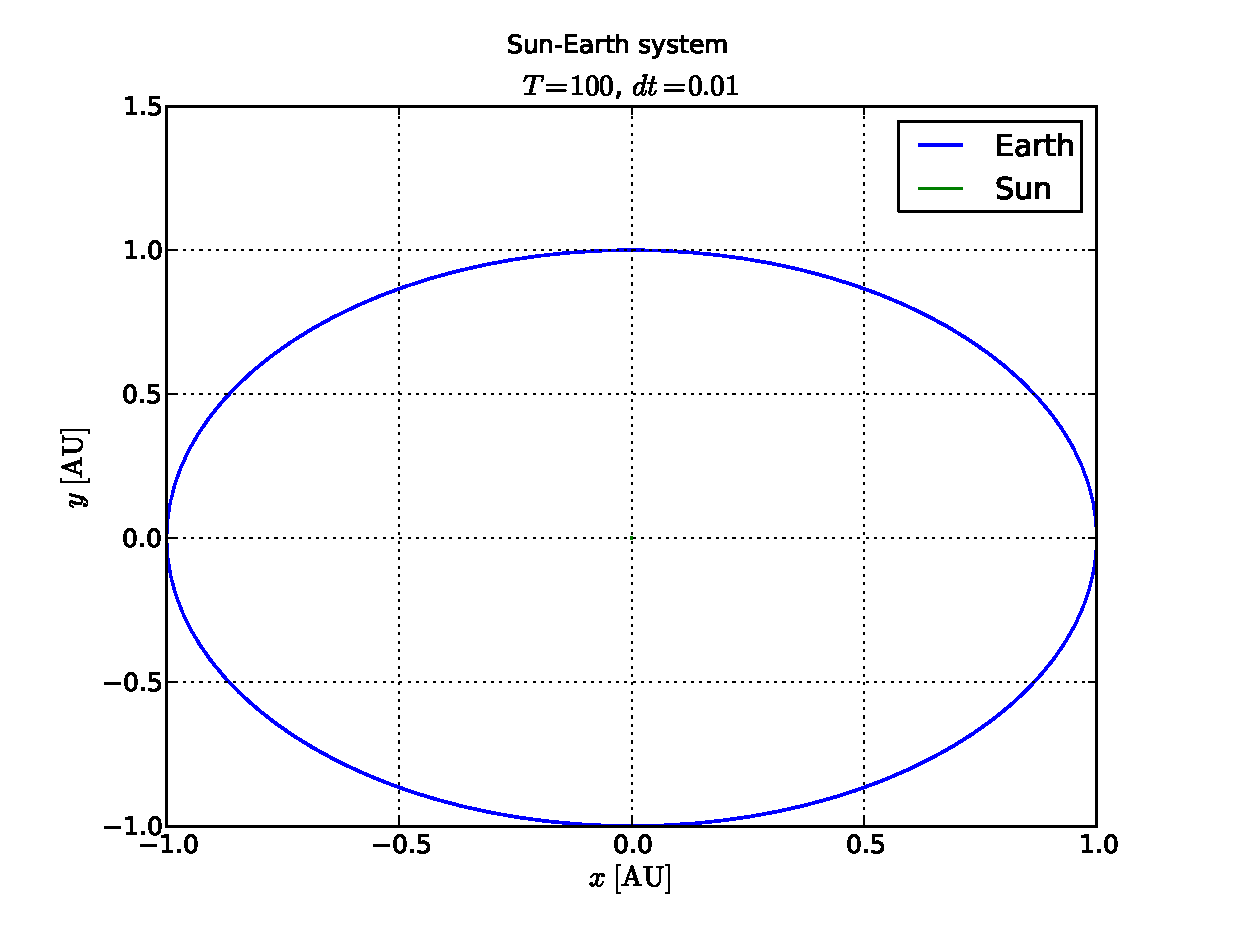
\includegraphics[width=0.8\textwidth]{figures/sun_earth_T100_dt1e-2}
	\caption{Earth's circular orbit around the Sun over a period of $T = 100$
	 years, with time step $dt = 0.01$. The initial values are 
	 $\mathbf{r} = [1,0]$, $\mathbf{v} = [0,1]$.}
	\label{fig:sunEarth-dt0.01}
\end{figure}
%
We notice that the orbit is circular (notice the axes), as expected, and quite
stable.
%By zooming far in on the center of Earth's orbit, we can see the
%movement of the Sun. See figure \refig{sun-zoom}.
%
%\begin{figure}[htpb]
%	\centering
%	\includegraphics[width=1.0\textwidth=]{figures/sun_zoom_dt1e-2.eps}
%	\caption{The Sun's movement due to the Earth. One semicircle is the Sun's
%	movement over the course of a year.}
%	\label{fig:sun-zoom}
%\end{figure}
%
Given that the orbit is circular, we expect the kinetic energy and the potential
energy to be conserved. The velocity is only expected to change its direction,
and not magnitude,
while orbiting, while the distance to the Sun is always the same. We can see
that this is the case in figure \refig{energycons}, which shows the energy
conservation.
%
\begin{figure}[htpb]
	\centering
	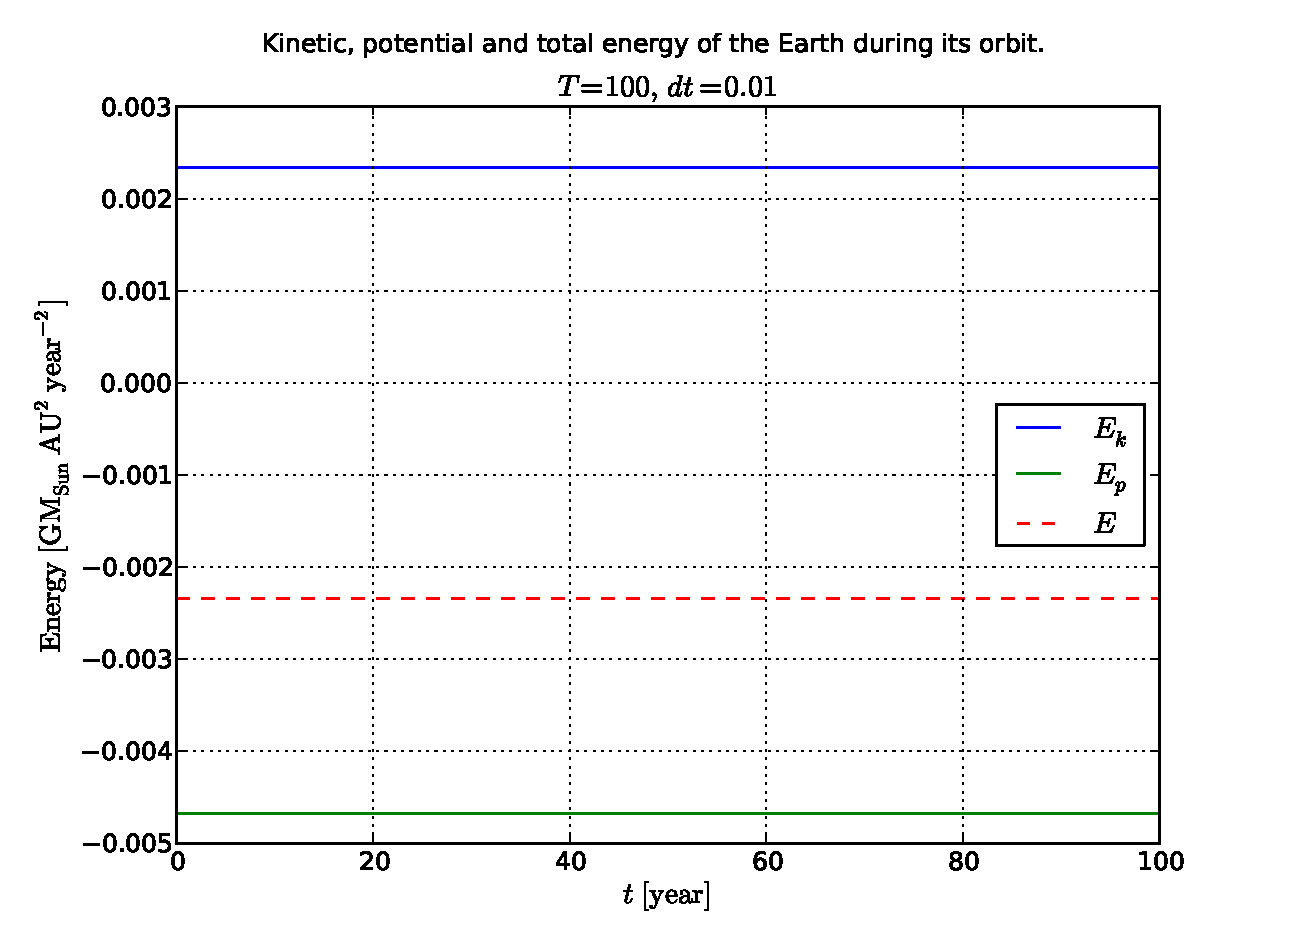
\includegraphics[width=0.8\textwidth]{figures/earth_energy_dt1e-2}
	\caption{The kinetic, potential and total energy of the Earth over a period
	of $T = 100$ years, with $dt = 0.01$. We see that both energy forms are
	conserved.}
	\label{fig:energycons}
\end{figure}
%
The angular momentum $\mathbf{L}$ is defined by
\begin{equation*}
	\mathbf{L} = \mathbf{r} \times\mathbf{p}
\end{equation*}
%
The velocity vector is always orthogonal to the position vector, such that the
direction of $\mathbf{L}$ is orthogonal to the $xy$-plane at all times. The
magnitude of the angular momentum vector is just the product $L =
rvM_{\text{Earth}}$, where $r$, $v$ are the magnitudes of the position vector
and velocity vector, respectively. We have shown above that these are constant,
so we expect the angular momentum of the Earth to be constant. The result is
shown in figure \refig{angmom}.
%
\begin{figure}[htpb]
	\centering
	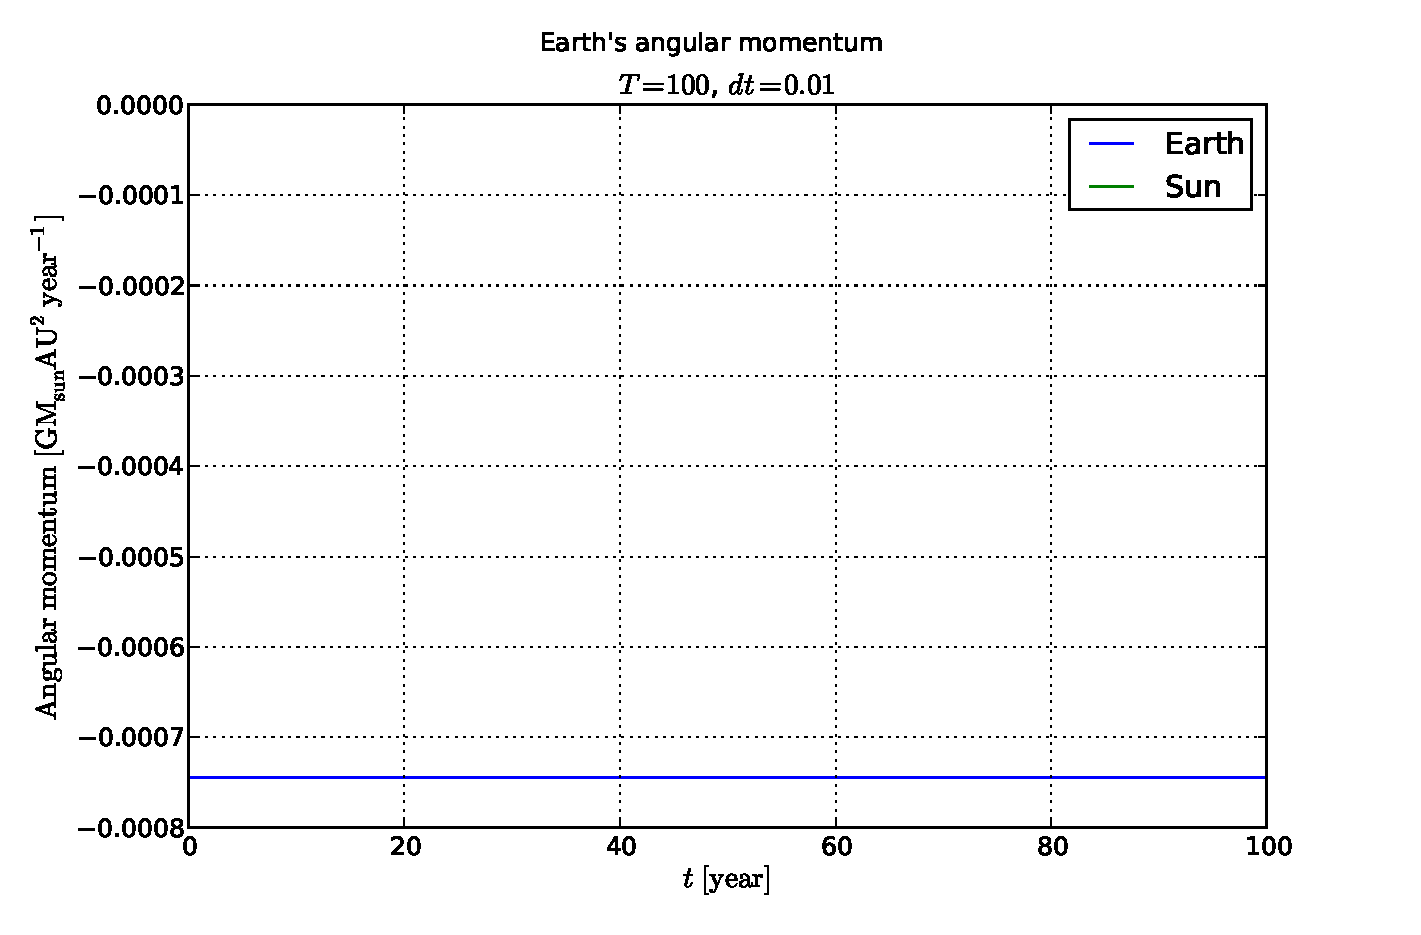
\includegraphics[width=0.8\textwidth]{figures/earth_angmom_dt1e-2}
	\caption{The angular momentum of the Earth, which is conserved throughout
	its orbit. Here shown for $T = 100$ years and $dt = 0.01$.}
	\label{fig:angmom}
\end{figure}
%
Let us now see what happens when we increase the time step. We increase
$dt$ by a factor of $10$, and consider Earth's orbit as shown in figure
\refig{sunEarth-dt0.1}.
%
\begin{figure}[htpb]
	\centering
	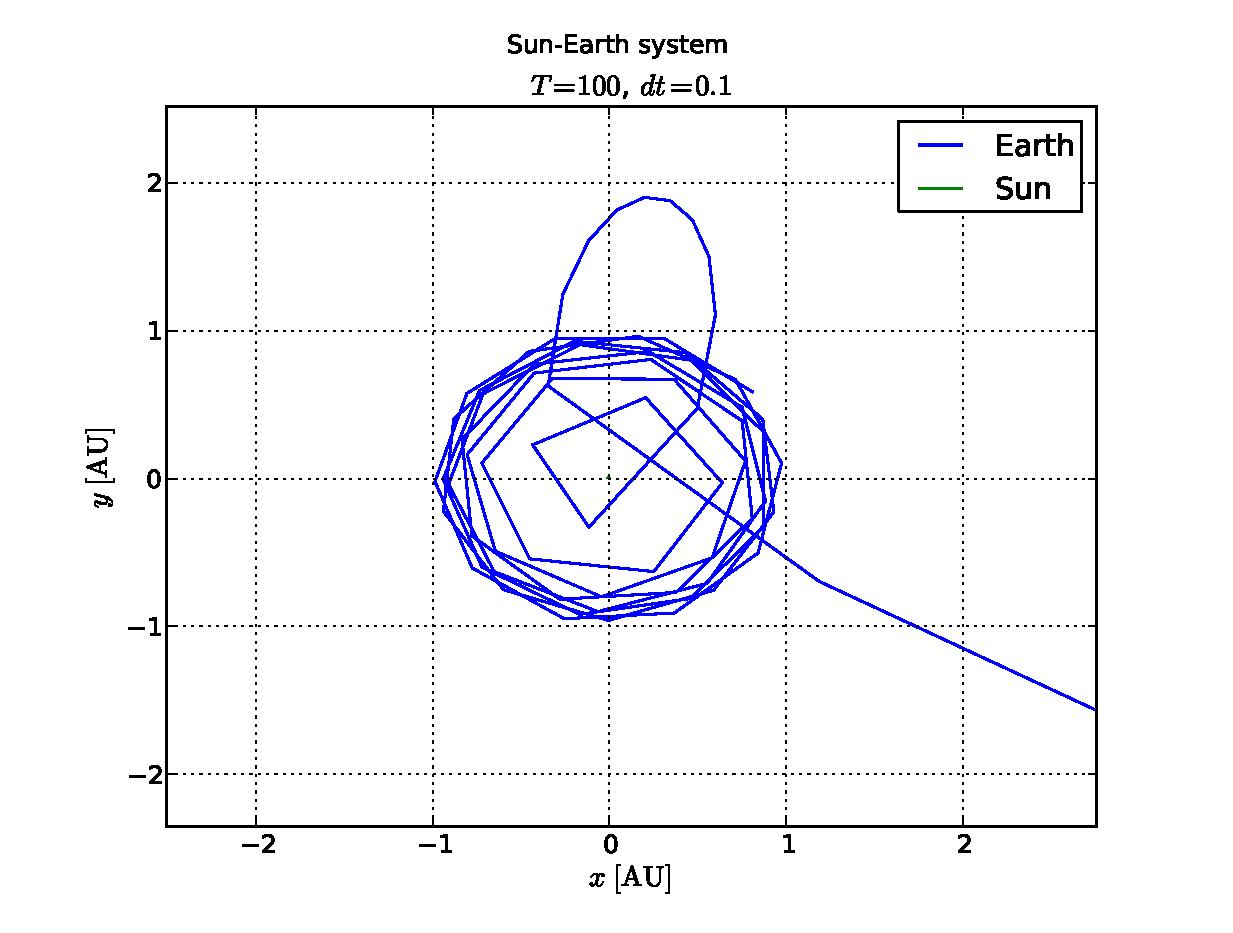
\includegraphics[width=0.8\textwidth]{figures/sun_earth_T100_dt1e-1_zoom}
	\caption{Earth's orbit around the sun for a time step $dt = 0.01$. We have
	zoomed in on the original figure to better see what happens before the Earth
	leaves orbit.}
	\label{fig:sunEarth-dt0.1}
\end{figure}
%
The trajectory starts out in a rough circular orbit, but loses energy as it
completes several orbits. At one point it is much closer to the Sun, such
that it gathers a higher velocity, resulting in a half loop outside the original
orbit. Upon returning, it again gathers a velocity higher than the escape
velocity, such that it leaves the solar system. The energy plot for this orbit
is included as well. See figure \refig{energyconstdt0.1}.
%
\begin{figure}[htpb]
	\centering
	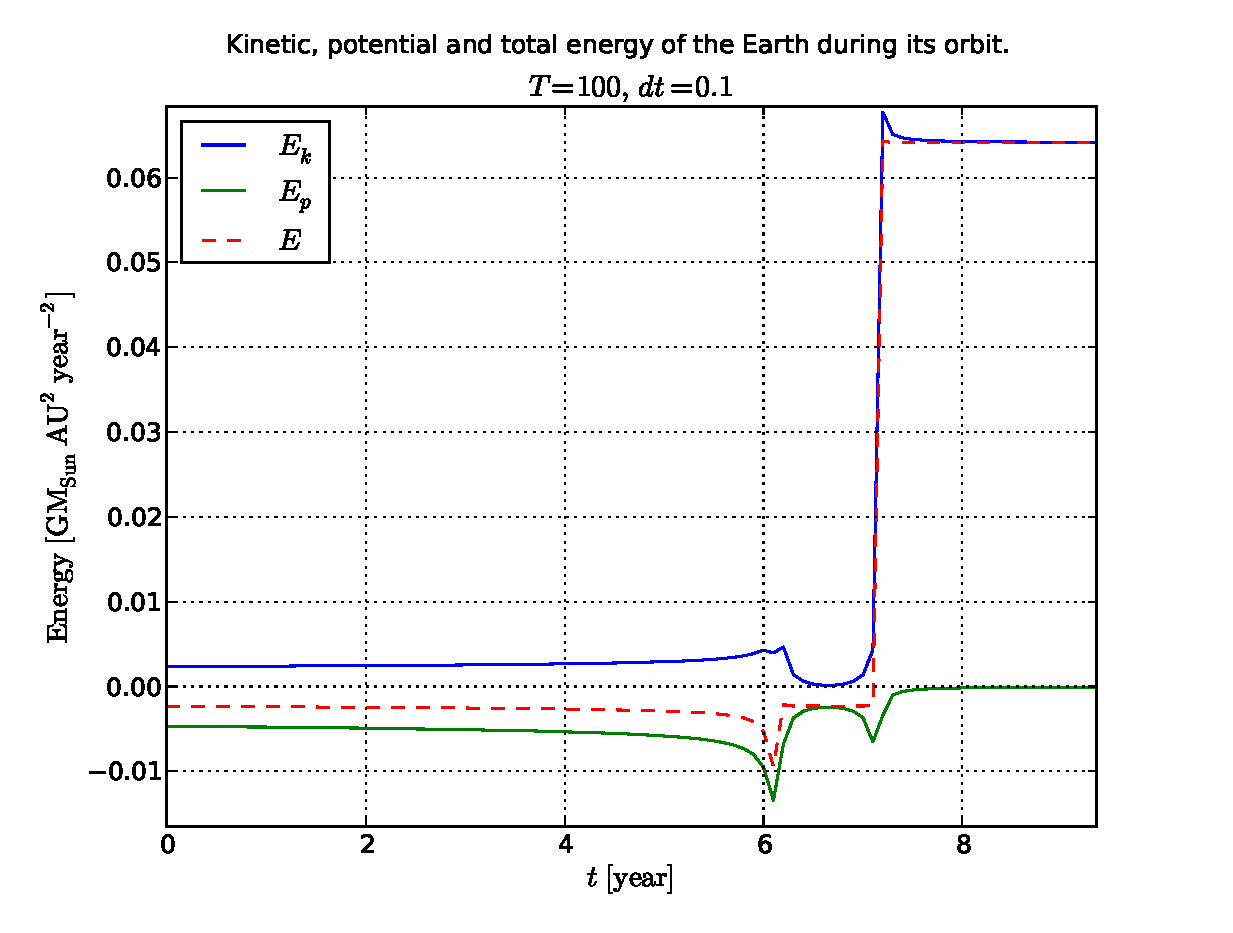
\includegraphics[width=0.8\textwidth]{figures/earth_energy_dt1e-1}
	\caption{Kinetic, potential and total energy for Earth while orbiting the
	Sun with time step $dt = 0.1$, over a course of $T = 100$ years.
	We have zoomed in on the relevant area.}
	\label{fig:energyconstdt0.1}
\end{figure}
%
We see that the potential energy is approximately zero after $t = 8$ years,
which means that Earth is free of the Sun's gravitational pull after this
time.

This is obviously a flaw in the RK4 method. It doesn't conserve energy for any
time step $dt$. Had we simulated the Sun-Earth system over a much longer time,
we would have seen the same thing happen for small time steps, like $dt =
10^{-2}$. 
A time step $dt = 0.1$ is big enough so that we can see the
method fail in the course of 100 years. We actually need less than 10 years
to see it fail, judging by figure \refig{energyconstdt0.1}. 
In some ways, a \emph{symplectic integrator} such as Euler-Cromer might have 
been better in such a simulation, because it conserves energy for any time step
$dt$. Using Euler-Cromer instead would however have a negative effect on the
accuracy.

We can test how large $dt$ can be before the method fails for a time span of 100
years. By trial and error we
find that a time step of about $dt = 5.5 \cdot 10^{-2}$ is just small enough to
prevent failure. See figure \refig{sunEarth-dt5.5e-2}.
%
\begin{figure}[htpb]
	\centering
	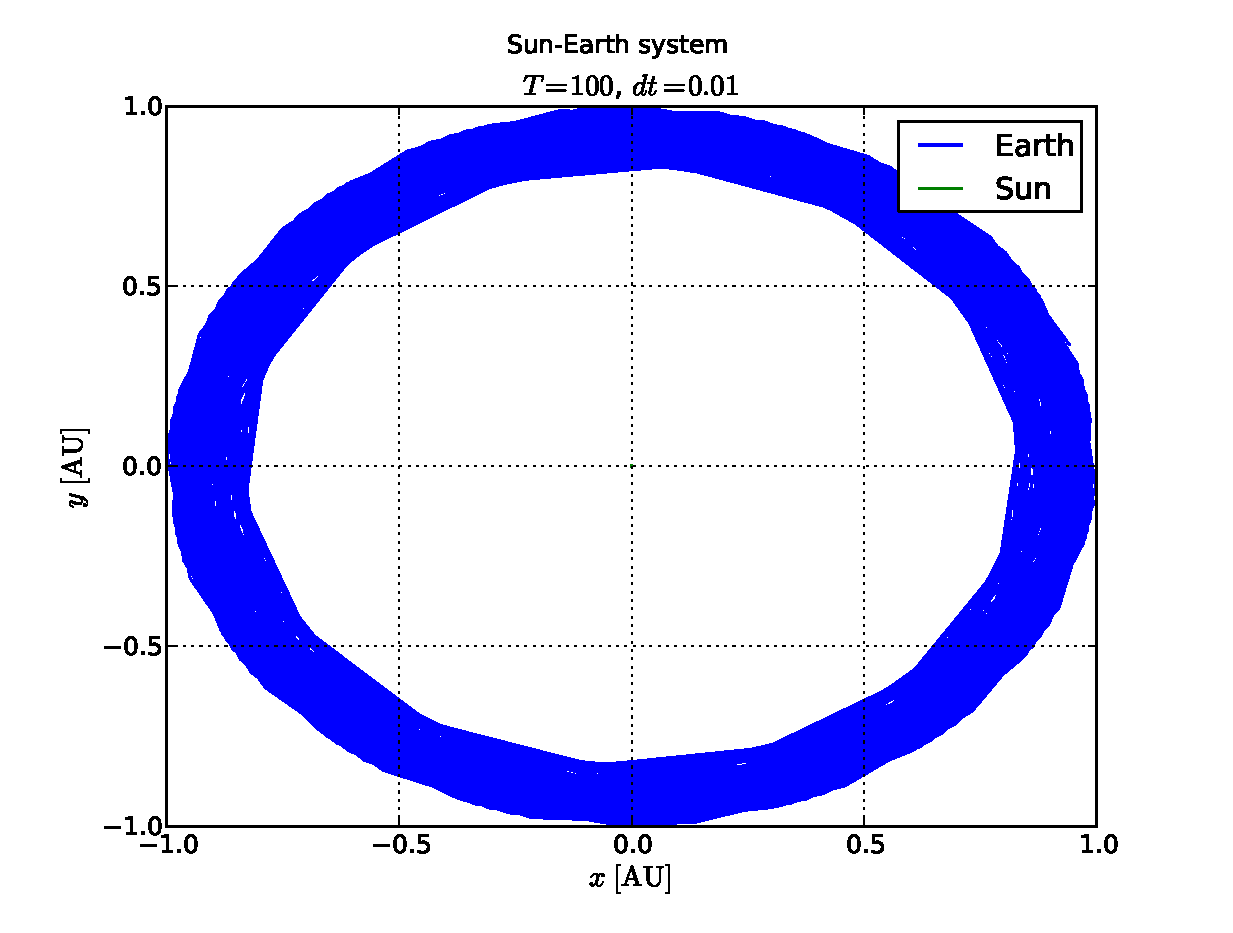
\includegraphics[width=0.8\textwidth]{figures/sun_earth_T100_dt5-5e-2}
	\caption{Earth's orbit about the Sun with $dt = 5.5 \cdot 10^{-2}$. The
	method is on the verge of failing for this time step. This is only valid for
	$T < 100$ years.}
	\label{fig:sunEarth-dt5.5e-2}
\end{figure}
%
Had we increased the time step to $dt = 6 \cdot 10^{-2}$, the method would have
failed. The limit then lies in the range $(5.5 - 6) \cdot 10^{-2}$.

\section{}
It is desirable that the total momentum $\mathbf{p}$ of all the celestial bodies should be $0$, like in equation \refeq{momentum_sum}. Then, the solar system will remain in place and the orbits will remain where they are. This makes it much easier to see what is acually going on when plotting and analyzing the result. In reality, the solar system \emph{do} have a total momentum, but in our model there is nothing moving relative to the solar system.

Gravity is a conservative force, so if $\mathbf{p} = 0$ is true at the initialization it should remain true always. If the initial velocites of all planets (and moons, asteroids, etc., if any) are given, one need simply to solve for the Sun's velocity $\mathbf{v}_\odot$ in equation \refeq{momentum_sun}, so that we get \refeq{momentum_sum2}, and set the velocity to this number in the program to make sure that $\mathbf{p} = 0$.
\begin{align}
	\label{eq:momentum_sum}
	\mathbf{p} =
	\mathbf{p}_\odot
	+ \mathbf{p}_\textrm{Mercury}
	+ \mathbf{p}_\textrm{Venus}
	+ \mathbf{p}_\textrm{Earth}
	+ \dots
	+ \mathbf{p}_\textrm{Pluto}
	&= 0 \\
	\label{eq:momentum_sun}
	m_\odot \mathbf{v}_\odot
	+ m_1 \mathbf{v}_1
	+ m_2 \mathbf{v}_2
	+ m_3 \mathbf{v}_3
	+ \dots
	+ m_N \mathbf{v}_N
	&= 0
\end{align}
\begin{equation}
    \label{eq:momentum_sum2}
    \mathbf{v}_\odot = - \frac{1}{m_\odot} \sum_i^N m_i \mathbf{v}_i
\end{equation}


To have origo be the center off mass for the solar system, we may first add the Sun and all planets with whichever positions we want, then calculate which position is the CM and subtract this position from every object, i.e. shifting the entire system so that the CM is placed in origo.
\begin{algorithmic}
    \State $ \mathbf{r}_{\textrm{CM}} = \sum_i^N m_i \mathbf{r}_i $
    \For{i = 1:N}
        \State $ \mathbf{r}_i = \mathbf{r}_i - \mathbf{r}_{\textrm{CM}} $
    \EndFor
\end{algorithmic}

The data on the planets' initial positions and velocities comes from NASA: \url{http://nssdc.gsfc.nasa.gov/planetary/factsheet/planet_table_ratio.html}. On this website there is no information on where each planet is at a given time, so we have just assumed that when $t=0$ every planet is on it's perihelion (and thus have it's greatest orbital velocity) and have given the perihelions arbitrary angular position. This leads to each planet's orbit being correct relative to the Sun, but not correct relative to the other planets (this is only a problem if our goal is to find the \emph{actual} state of the solar system at various times). The general picture, however, is correct. E.g. we can see details such as Jupiter tugging on nearby planets and Neptune's and Pluto's orbits crossing eachother.



\end{document}
